\documentclass[tikz,margin=1mm]{standalone}
\usepackage{xcolor}
 \usetikzlibrary{arrows.meta,chains, decorations.pathreplacing}



\begin{document}
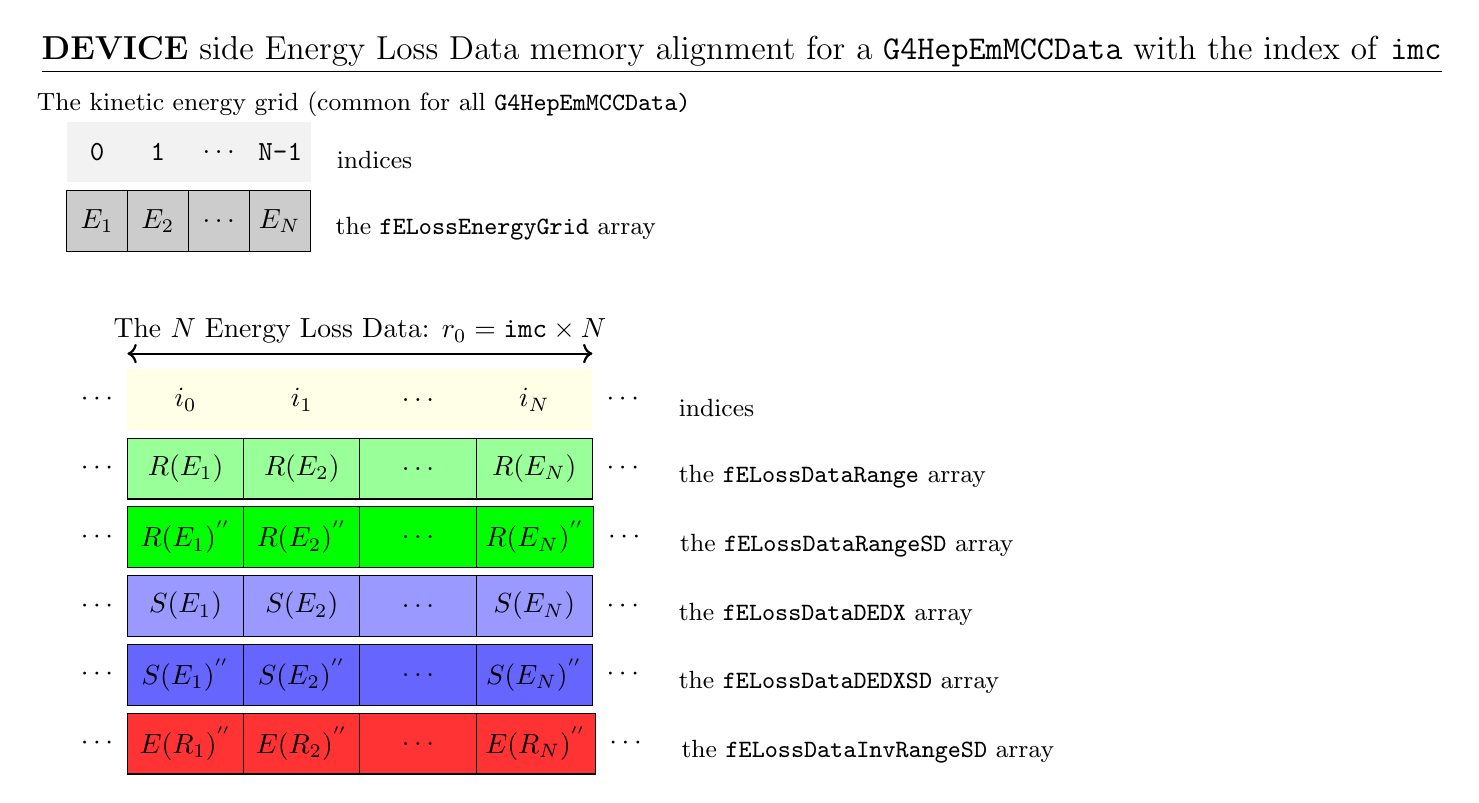
\begin{tikzpicture}[
   start chain       = going right,
   node distance = 0pt,
   %
   noStyle/.style  = {draw=none, minimum width=2.2em, minimum height=2.2em, outer sep=0pt, font=\ttfamily, on chain},
   % 
   eiStyle/.style  = {draw=none, minimum width=2.2em, minimum height=2.2em, outer sep=0pt, font=\ttfamily, on chain, fill=gray!10},
   eStyle/.style   = {draw, minimum width=2.2em, minimum height=2.2em, outer sep=0pt, on chain, fill=gray!40},
   %
   iStyle/.style  = {draw=none, minimum width=4.2em, minimum height=2.2em, outer sep=0pt, font=\ttfamily, on chain, fill=yellow!10},
   %
   rStyle/.style   = {draw, minimum width=4.2em, minimum height=2.2em, outer sep=0pt, on chain, fill=green!40},
   rSDStyle/.style   = {draw, minimum width=4.2em, minimum height=2.2em, outer sep=0pt, on chain, fill=green!100},
   %
   sSDStyle/.style  = {draw, minimum width=4.2em, minimum height=2.2em, outer sep=0pt, font=\ttfamily, on chain, fill=blue!60},
   sStyle/.style   = {draw, minimum width=4.2em, minimum height=2.2em, outer sep=0pt, on chain, fill=blue!40},
   %
   irStyle/.style  = {draw, minimum width=4.2em, minimum height=2.2em, outer sep=0pt, font=\ttfamily, on chain, fill=red!80},
   %
   imcStyle/.style  = {draw=none, minimum width=4.2em, minimum height=2.2em, outer sep=0pt, font=\ttfamily, on chain, fill=yellow!30},
   mcStyle/.style  = {draw, minimum width=4.2em, minimum height=2.2em, outer sep=0pt, font=\ttfamily, on chain, fill=yellow!80},
  ]

    \begin{scope}[start chain=EGRIDINDX going right];
        \node [eiStyle] (Ei1) {0};
        \node [eiStyle] (Ei2) {1};
        \node [eiStyle] (Ei3) {$\ldots$};
        \node [eiStyle] (Ei4) {N-1};
    \end{scope}

    \node[anchor=north, at={([yshift=+12mm,xshift=+78mm]EGRIDINDX-1.north east)}] {\large {\underline{\textbf{DEVICE} side Energy Loss Data memory alignment  for a \texttt{G4HepEmMCCData}  with the index of \texttt{imc}} }};
    
    \node[anchor=north, at={([yshift=+5mm,xshift=+30mm]EGRIDINDX-1.north east)}] {\small {The kinetic energy grid (common for all \texttt{G4HepEmMCCData)}}};

    \begin{scope}[start chain=EGRID going right];
        \node [eStyle, anchor=north, at={([yshift=-1mm]EGRIDINDX-1.south)}] (E1) {$E_1$};
        \node [eStyle] (E2) {$E_2$};
        \node [eStyle] (E3) {$\ldots$};
        \node [eStyle] (E4) {$E_N$};
    \end{scope}

    \node[anchor=west, at={([yshift=-1mm,xshift=2mm]EGRIDINDX-4.east)}] {\small {indices}};
    \node[anchor=west, at={([yshift=-1mm,xshift=2mm]EGRID-4.east)}] {\small {the \texttt{fELossEnergyGrid} array}};





    \begin{scope}[start chain=INDX going right];
        \node [noStyle, anchor=north, at={([yshift=-15mm]EGRID-1.south)}] (I1) {$\cdots$};
        \node [iStyle] (I2) {$i_0$};
        \node [iStyle] (I3) {$i_1$};
        \node [iStyle] (I4) {$\ldots$};
        \node [iStyle] (I5) {$i_N$};
        \node [noStyle] (I6) {$\cdots$};
    \end{scope}
     \draw[<->, thick] ([yshift=+2mm]INDX-2.north west) -- node[above] {The $N$ Energy Loss Data: $r_0=\texttt{imc}\times N$} ([yshift=+2mm]INDX-5.north east);
     \node[anchor=west, at={([yshift=-1mm,xshift=2mm]INDX-6.east)}] {\small {indices}};
    
    \begin{scope}[start chain=RANGE going right];
        \node [noStyle, anchor=north, at={([yshift=-1mm]INDX-1.south)}] (R1) {$\cdots$};
        \node [rStyle] (R2) {$R(E_1)$};
        \node [rStyle] (R3) {$R(E_2)$};
        \node [rStyle] (E4) {$\ldots$};
        \node [rStyle] (R5) {$R(E_N)$};
        \node [noStyle] (R6) {$\cdots$};
    \end{scope}
    \node[anchor=west, at={([yshift=-1mm,xshift=2mm]RANGE-6.east)}] {\small {the \texttt{fELossDataRange} array}};

    \begin{scope}[start chain=SDRANGE going right];
        \node [noStyle, anchor=north, at={([yshift=-1mm]RANGE-1.south)}] (RSD1) {$\cdots$};
        \node [rSDStyle] (RSD2) {$R(E_1)^{''}$};
        \node [rSDStyle] (RSD3) {$R(E_2)^{''}$};
        \node [rSDStyle] (RSD4) {$\ldots$};
        \node [rSDStyle] (RSD5) {$R(E_N)^{''}$};
        \node [noStyle] (RSD6) {$\cdots$};
    \end{scope}
    \node[anchor=west, at={([yshift=-1mm,xshift=2mm]SDRANGE-6.east)}] {\small {the \texttt{fELossDataRangeSD} array}};

    \begin{scope}[start chain=SP going right];
        \node [noStyle, anchor=north, at={([yshift=-1mm]SDRANGE-1.south)}] (S1) {$\cdots$};
        \node [sStyle] (S2) {$S(E_1)$};
        \node [sStyle] (S3) {$S(E_2)$};
        \node [sStyle] (S4) {$\ldots$};
        \node [sStyle] (S5) {$S(E_N)$};
        \node [noStyle] (S6) {$\cdots$};
    \end{scope}
     \node[anchor=west, at={([yshift=-1mm,xshift=2mm]SP-6.east)}] {\small {the \texttt{fELossDataDEDX} array}};

    \begin{scope}[start chain=SPSD going right];
        \node [noStyle, anchor=north, at={([yshift=-1mm]SP-1.south)}] (SSD1) {$\cdots$};
        \node [sSDStyle] (SSD2) {$S(E_1)^{''}$};
        \node [sSDStyle] (SSD3) {$S(E_2)^{''}$};
        \node [sSDStyle] (SSD4) {$\ldots$};
        \node [sSDStyle] (SSD5) {$S(E_N)^{''}$};
        \node [noStyle] (SSD6) {$\cdots$};
    \end{scope}
     \node[anchor=west, at={([yshift=-1mm,xshift=2mm]SPSD-6.east)}] {\small {the \texttt{fELossDataDEDXSD} array}};


    \begin{scope}[start chain=IR going right];
        \node [noStyle, anchor=north, at={([yshift=-1mm]SPSD-1.south)}] (IR1) {$\cdots$};
        \node [irStyle] (IR2) {$E(R_1)^{''}$};
        \node [irStyle] (IR3) {$E(R_2)^{''}$};
        \node [irStyle] (IR4) {$\ldots$};
        \node [irStyle] (IR5) {$E(R_N)^{''}$};
        \node [noStyle] (IR6) {$\cdots$};
    \end{scope}
     \node[anchor=west, at={([yshift=-1mm,xshift=2mm]IR-6.east)}] {\small {the \texttt{fELossDataInvRangeSD} array}};





%    \begin{scope}[start chain=IMCINDX going right];
%        \node [imcStyle, anchor=west, at={([yshift=+40mm,xshift=40mm]SDRANGE-4.east)}] (IMC1) {$\texttt{0}$};
%        \node [imcStyle] (IMC2) {$\texttt{1}$};
%        \node [imcStyle] (IMC3) {$\ldots$};
%        \node [imcStyle] (IMC4) {$\texttt{imc}$};
%        \node [imcStyle] (IMC5) {$\ldots$};
%        \node [imcStyle] (IMC6) {$\texttt{M}$};
%    \end{scope}
%   \draw[<->, thick] ([yshift=+2mm]IMCINDX-1.north west) -- node[above] {The $M$ \texttt{G4HepEmMCCData} material - cuts data indices} ([yshift=+2mm]IMCINDX-6.north east);

 %   \begin{scope}[start chain=MCINDX going right];
 %       \node [mcStyle, anchor=north, at={([yshift=-1mm]IMCINDX-1.south)}] (MC1) {$\cdot$};
 %       \node [mcStyle] (MC2) {$\cdot$};
%        \node [mcStyle] (MC3) {$\ldots$};
 %       \node [mcStyle] (MC4) {$\texttt{imc}$};
 %       \node [mcStyle] (MC5) {$\ldots$};
 %       \node [mcStyle] (MC6) {$\texttt{M}$};
 %   \end{scope}



\end{tikzpicture}
\end{document}